\documentclass{moderncv}

\moderncvtheme{classic} 
\moderncvcolor{blue}

\definecolor{dark-gray}{gray}{0.20}
                                
\usepackage[utf8]{inputenc}                      
\usepackage[scale=0.75]{geometry}
\usepackage{import}
\usepackage{multicol}
\usepackage{graphicx}
\usepackage{float}
\usepackage[absolute,overlay]{textpos}
\usepackage{lipsum}
\usepackage{etoolbox}
\usepackage[T1]{fontenc}
\usepackage{xcolor}
\usepackage{fontawesome}
\usepackage{fontspec}
\usepackage{color}
\usepackage{tikz}
\usepackage{xpatch}
\usepackage{color,soul}

\usetikzlibrary{shapes.misc,shadows}
\usetikzlibrary{calc,shapes}

\setul{0.5ex}{0.2ex}
\definecolor{Blue}{rgb}{0,0.0,1}
\setulcolor{Blue}

\name{\LARGE{\textcolor{blue}{\textsc{PRASHANT}}}}{\LARGE{\textcolor{blue}{\textsc{KUMAR}}}} 
\address{Bengaluru Karnataka, India}{Bengaluru - 560025}
\social[linkedin]{prashantcse}
\phone[mobile]{\faMobilePhone \hspace{7pt}+(91) - 9694725810} 
\social[github]{PrashantPST}
\email{prashantkr.kumar88@gmail.com}


\renewcommand*{\mobilephonesymbol}{}
\renewcommand*{\cventry}[7][.25em]{%
  \cvitem[#1]{#2}{%
    {\bfseries#3}%
%   \ifthenelse{\equal{#4}{}}{}{, {\slshape#4}}% I changed this line (with comma) ...
    \ifthenelse{\equal{#4}{}}{}{ {\slshape#4}}% ... into this one (without comma).
    \ifthenelse{\equal{#5}{}}{}{ {\slshape#5}}%
    \ifthenelse{\equal{#6}{}}{}{ {\slshape#6}}%
    .\strut%
    \ifx&#7&%
      \else{\newline{}\begin{minipage}[t]{\linewidth}\small#7\end{minipage}}\fi}}
            
\begin{document}

\makecvtitle

\section{\textsc{Snapshot}}

\vspace{2pt}

\small{A software engineer currently engaged with MILVIK India having ten months of professional experience. I did my M.Tech. From NIT Jaipur and having a B.Tech. From Uttarakhand Technical University.}

\vspace{4pt}

\section{\textsc{Work Experience}}

\cventry{Feb 2018--Present}{Software Engineer}{MILVIK India}{}
\small{\begin{itemize}
\item{\ul{L2 Support Month End Automation -}}\\
A web application developed for providing a dashboard for L2 support team for their month-end tasks.
\begin{itemize}
\item Used Django for backend service and its templating engine for rendering UI.
\item Remove the manual procedures which were error prone.
\item It Reduces the time from many hours to just a few minutes.
\item All database operations ran in a transaction; no inconsistent
state of the database on failure(app).
\end{itemize}
\item{\ul{Data Migration Service -}}\\
Migration service(a service which is part of a stack of services) in a spring-backend microservice architecture.
\begin{itemize}
\item A spring boot enabled service integrated with Kafka.
\item A producer-consumer model where producer listens to the table on our one end platform and consumer consumes the same and stores at another end of a platform.
\item Producer(Maxwell's daemon), an application that reads MySQL binlogs and writes row updates to Kafka.
\end{itemize}
\end{itemize}}
\vspace{5pt}

\cventry{Nov 2017--Jan 2018}{Software Engineer Trainee}{CodeHall Technology Pvt. Ltd. Bengaluru}{}
\small{\begin{itemize}
\item{\ul{College Search -}}\\
A web app for helping users(with varied roles) from the beginning of searching colleges to the seat allocation and college orientation for the students of different disciplines.
\begin{itemize}
\item Django backend microservice architecture in conjunction with React for UI.
\item Discussion on the Database and API design of each service built by team members.
\item Write the code for StudentProfile and News\&Events services.
\end{itemize}
\end{itemize}}

\thispagestyle{empty} 

\section{\textsc{Projects}}

\vspace{3pt}

\begin{itemize}

\item{\textbf{A Blog Web App}} 
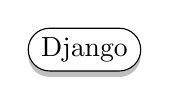
\begin{tikzpicture}[baseline=(char.base)]
\node(char)[draw,fill=white,
  shape=rounded rectangle,
  drop shadow={opacity=.5,shadow xshift=0pt},
  minimum width=0.7cm]
  {Django};
\end{tikzpicture}
\vspace{3pt}

A blog web application where registered users can write their blog and could post it. Any anonymous users can view all blogs and could also filter blogs for a specific user. A registered user could modify/ delete their blog only. 

\vspace{2pt}

Repo Link: \url{https://github.com/PrashantPST/django-blog.git}

\vspace{3pt}

\item{\textbf{Swiss Tournament Web App}} 
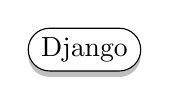
\begin{tikzpicture}[baseline=(char.base)]
\node(char)[draw,fill=white,
  shape=rounded rectangle,
  drop shadow={opacity=.5,shadow xshift=0pt},
  minimum width=0.7cm]
  {Django};
 
\end{tikzpicture}

\begin{tikzpicture}[baseline=(char.base)]
\node(char)[draw,fill=white,
  shape=rounded rectangle,
  drop shadow={opacity=.5,shadow xshift=0pt},
  minimum width=0.7cm]
  {React};
\end{tikzpicture}
\vspace{3pt}

In a Swiss tournament, players get never eliminated. Instead, players get paired in every round based on their scores. The two closest score player would clash for the next round, and the winner is the player who earns the most points at the end of the tournament. 

\vspace{2pt}

The entire project has two sub-projects, one as a front-end (which is a React App), and the other one as aback-end (a Django project).

\vspace{2pt}

Front End Repo: \url{https://github.com/PrashantPST/swiss-tournament-frontend.git}

\vspace{1pt}

Back End Repo: \url{https://github.com/PrashantPST/swiss-tournament-backend.git}

\vspace{3pt}


\item{\textbf{Masters Thesis} SAFETY: Early Detection \& Mitigation of TCP
SYN Flood Utilizing Entropy in Software Defined Networking.

\vspace{3pt}

\small{This thesis presents SAFETY, a novel solution for the early detection and mitigation of TCP SYN flood harnessing the programming and wide visibility approach of SDN using entropy for destination IP with the attribute of TCP flags.}}

\vspace{4pt}

\end{itemize}

\vspace{2pt}

\section{\textsc{Publication}}

\vspace{2pt}

\begin{itemize}
\item{\textbf{SAFETY}: Early Detection and Mitigation of TCP SYN Flood Utilizing Entropy in SDN}\\
\textbf{Publication/Publisher} - IEEE Transactions on Network and Service Management \\
\textbf{Publication date} - 2018-07-31 \\
\textbf{Publication URL} - \url{https://ieeexplore.ieee.org/abstract/document/8423699/}
\end{itemize}

\section{\textsc{Technical Stack}}

\vspace{2pt}

\begin{itemize}

\item \textbf{Programming Language:} 
\begin{tikzpicture}[baseline=(char.base)]
\node(char)[draw,fill=white,
  shape=rounded rectangle,
  drop shadow={opacity=.5,shadow xshift=0pt},
  minimum width=0.7cm]
  {Python};
\end{tikzpicture}

\begin{tikzpicture}[baseline=(char.base)]
\node(char)[draw,fill=white,
  shape=rounded rectangle,
  drop shadow={opacity=.5,shadow xshift=0pt},
  minimum width=0.7cm]
  {Java};
\end{tikzpicture}

\begin{tikzpicture}[baseline=(char.base)]
\node(char)[draw,fill=white,
  shape=rounded rectangle,
  drop shadow={opacity=.5,shadow xshift=0pt},
  minimum width=0.7cm]
  {JavaScript};
\end{tikzpicture}
\vspace{3pt}
\item \textbf{Web Framework:}
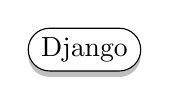
\begin{tikzpicture}[baseline=(char.base)]
\node(char)[draw,fill=white,
  shape=rounded rectangle,
  drop shadow={opacity=.5,shadow xshift=0pt},
  minimum width=0.7cm]
  {Django};
\end{tikzpicture}

\begin{tikzpicture}[baseline=(char.base)]
\node(char)[draw,fill=white,
  shape=rounded rectangle,
  drop shadow={opacity=.5,shadow xshift=0pt},
  minimum width=0.7cm]
  {Spring};
\end{tikzpicture}

\vspace{3pt}

\item \textbf{JavaScript Library}

\begin{tikzpicture}[baseline=(char.base)]
\node(char)[draw,fill=white,
  shape=rounded rectangle,
  drop shadow={opacity=.5,shadow xshift=0pt},
  minimum width=0.7cm]
  {React};
\end{tikzpicture}

\vspace{3pt}

\item \textbf{Database:} 

 \vspace{1pt}
    \begin{itemize}
    \item \textbf{Relational:} 
\begin{tikzpicture}[baseline=(char.base)]
\node(char)[draw,fill=white,
  shape=rounded rectangle,
  drop shadow={opacity=.5,shadow xshift=0pt},
  minimum width=0.7cm]
  {MySQL};
\end{tikzpicture}
\vspace{2pt}
\item \textbf{Document:} 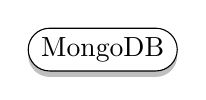
\begin{tikzpicture}[baseline=(char.base)]
\node(char)[draw,fill=white,
  shape=rounded rectangle,
  drop shadow={opacity=.5,shadow xshift=0pt},
  minimum width=0.7cm]
  {MongoDB};
\end{tikzpicture}
    \end{itemize}
    
\vspace{3pt}

\item \textbf{Streaming Platform:} 
\begin{tikzpicture}[baseline=(char.base)]
\node(char)[draw,fill=white,
  shape=rounded rectangle,
  drop shadow={opacity=.5,shadow xshift=0pt},
  minimum width=0.7cm]
  {Apache Kafka};
\end{tikzpicture}

\vspace{3pt}

\item \textbf{Version Control System:} 
\begin{tikzpicture}[baseline=(char.base)]
\node(char)[draw,fill=white,
  shape=rounded rectangle,
  drop shadow={opacity=.5,shadow xshift=0pt},
  minimum width=0.7cm]
  {Git};
\end{tikzpicture}

\vspace{3pt}

\thispagestyle{empty}

\end{itemize}

\vspace{4pt}

\section{\textsc{Accolades}}

\vspace{1pt}


\begin{itemize}

\item Secured AIR 653 in GATE 2015.

\end{itemize}

\section{\textsc{Education}}

\vspace{3pt}

\begin{itemize}

\item[]{\cventry{2015--2017}{M.Tech. in Computer Engineering}{Malaviya National Institute of Technology}{Jaipur}{7.33 CGPA}{}}

\item[]{\cventry{2010--2014}{B.Tech. in Computer Science \& Engineering}{Govind Ballabh Pant Institute of Engineering \& Technology}{Uttarakhand}{\textit{76.04 \%(Honours)}}{}}

\end{itemize}

\thispagestyle{empty}

\vspace{3pt}



\end{document}